\documentclass[final,hyperref={pdfpagelabels=false}]{beamer}
\usepackage{grffile}
\mode<presentation>{\usetheme{UoL}}
\usepackage[english]{babel}
\usepackage[T1]{fontenc} 
\usepackage[utf8]{inputenc}
\usepackage{amsmath,amsthm, amssymb, latexsym}
\usepackage[scaled=0.98]{helvet}
%\usepackage{times}\usefonttheme{professionalfonts}  % obsolete
%\usefonttheme[onlymath]{serif}
\boldmath
\usepackage[orientation=landscape,size=a0,scale=0.9]{beamerposter}
\usepackage{wrapfig}
\usepackage{comment}
% change list indention level
\setdefaultleftmargin{5em}{}{}{}{}{}

\usepackage[
backend=biber,
natbib=true,
style=numeric,
sorting=none]{biblatex}

\addbibresource{bagneux-14.bib}

%\usepackage{snapshot} % will write a .dep file with all dependencies, allows for easy bundling

\usepackage{array,booktabs,tabularx}
\newcolumntype{Z}{>{\centering\arraybackslash}X} % centered tabularx columns
\newcommand{\pphantom}{\textcolor{ta3aluminium}} % phantom introduces a vertical space in p formatted table columns??!!
\usepackage{parcolumns}

\listfiles

%%%%%%%%%%%%%%%%%%%%%%%%%%%%%%%%%%%%%%%%%%%%%%%%%%%%%%%%%%%%%%%%%%%%%%%%%%%%%%%%%%%%%%
\graphicspath{{figures/}}
 
\title{\huge Towards Distributed, Behaviour-Based Trust for Autonomous Submarine Teams}
\author{Andrew Bolster, Prof. Alan Marshall, Prof. Jean-Guy Fontaine }
\institute[UoL]{Advanced Networks Research Group, University of Liverpool, UK}
\date[03/07/14]{July 3rd, 2014}

%%%%%%%%%%%%%%%%%%%%%%%%%%%%%%%%%%%%%%%%%%%%%%%%%%%%%%%%%%%%%%%%%%%%%%%%%%%%%%%%%%%%%%


\def\colwidth{0.2\linewidth}

\usecaptiontemplate{
\small
\structure{\insertcaptionname~\insertcaptionnumber:}
\insertcaption
} 
%%%%%%%%%%%%%%%%%%%%%%%%%%%%%%%%%%%%%%%%%%%%%%%%%%%%%%%%%%%%%%%%%%%%%%%%%%%%%%%%%%%%%%
\begin{document}
\begin{frame}[fragile]
  \begin{columns}[T]
    % ---------------------------------------------------------%
    % Set up a column 
    \begin{column}{\colwidth}
      \begin{beamercolorbox}[center,wd=\textwidth]{postercolumn}
        \begin{minipage}[T]{.98\textwidth}  % tweaks the width, makes a new \textwidth
          \parbox[t]{\textwidth}{ % must be some better way to set the the height, width and textwidth simultaneously
          % Since all columns are the same length, it is all nice and tidy.  You have to get the height empirically
          % ---------------------------------------------------------%
          % fill each column with content            
          %%%%%%%%%%%%
          \begin{block}{Project Background}

            \begin{itemize}
              \item Project launched at QUB ECIT in 2011 under the DSTL/DGA Anglo French Defence Research Group PhD Programme  \item What lessons from the Mobile Ad Hoc Network (MANET) space can be transferred to the marine environment?
              \item Teams of 3 - 16 Autonomous Underwater Vehicles (AUVs) with Mine countermeasures, Hydrography, and Patrol Capabilities (MHPC)
              \item Defence focus, assumption of highly capable enemy attempting to compromise communications / operations
              \item Primary Simulation/Analysis work done in 12/13
              \item Moved to UoL Oct 13 after 2 mth placement @ DSTL PDW Naval Systems / Information Systems departments.
              \item CDE Project on Precision Timing for Collaborative Acoustic Positioning with NPL/Plextek
            \end{itemize}
          \end{block}

          %%%%%%%%%%%%
          \begin{block}{Introduction}
            \emph{Aim of project}: To use physical behaviours and observations to assess and maintain trust within mobile, marine, ad-hoc networks

            \vspace{0.3\baselineskip}

            Small fleets of AUVs (\emph{Autonomous Underwater Vehicles}) will be expected to operate in isolated environments.
            \vspace{0.3\baselineskip}

            This requires an auditable sense of trust within the remote intra-fleet communications networks, incorporating
            \begin{itemize}
              \item Communications Activity
              \item Mission Suitability/Capability
              \item Behavioural Monitoring
            \end{itemize}

            \vspace{0.3\baselineskip}

            The use of centrally coordinated trust models presents a single point of failure.

            \vspace{0.3\baselineskip}

            Secure communication in marine environments is expensive and time consuming; adopting a decentralised form of trust assurance will reduce these costs by localising the per-node security environment.

            \begin{figure}[h]
              \centering
              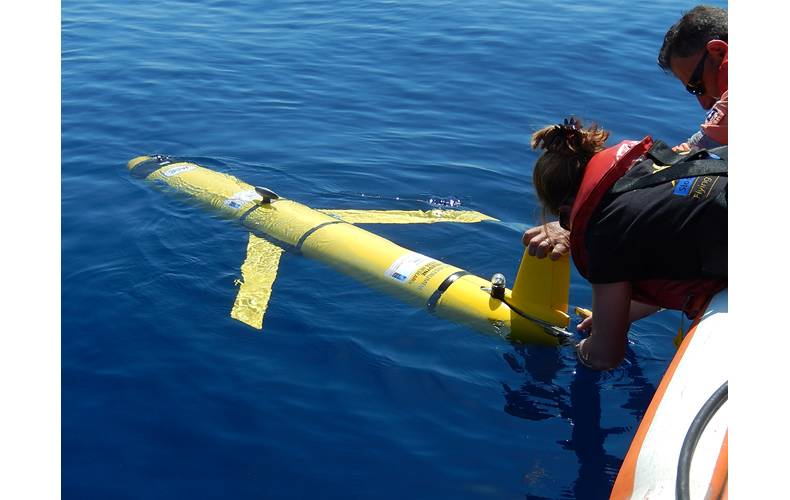
\includegraphics[width=0.6\linewidth]{remus100cmre}
              \vspace{1ex}
              \caption{REMUS 100 AUV, as deployed at CMRE, a potential target platform for this work}
            \end{figure}



          \end{block}
          %%%%%%%%%%%%
          \begin{block}{Trust}
            Trust is:
            \begin{itemize}
              \item \emph{The expectation of an actor performing a certain task or range of tasks within a certain confidence or probability}
              \item a belief on the reliability of an entity
              \item based on both direct and indirect historical experience
            \end{itemize}
            \vspace{0.3\baselineskip}

            Individual trust opinions are shared within the network concerning a range of activities:
            \begin{itemize}
              \item Transmission Relaying (Local and/or Backhaul)
              \item Position Relaying
              \item Reporting Accuracy
            \end{itemize}
            \vspace{0.3\baselineskip}

            These Trust opinions also apply to extra-fleet entities, such as surface platforms, submarine comms links, and coastal stations, allowing the fleet to collaboratively form an opinion of these actors.

          \end{block}
          }
        \end{minipage}
      \end{beamercolorbox}
    \end{column}
    % ---------------------------------------------------------%
    % end the column

    % ---------------------------------------------------------%
    % Set up a column 
    \begin{column}{\colwidth}
      \begin{beamercolorbox}[center,wd=\textwidth]{postercolumn}
        \begin{minipage}[T]{.98\textwidth} % tweaks the width, makes a new \textwidth
          \parbox[t]{\textwidth}{ % must be some better way to set the the height, width and textwidth simultaneously
          % Since all columns are the same length, it is all nice and tidy.  You have to get the height empirically
          % ---------------------------------------------------------%
          % fill each column with content
          %%%%%%%%%%%%
          \begin{block}{Trust Management Frameworks (TMFs)}
            TMFs are protocols designed to provide information regarding the estimated future states and operations of nodes within networks
            \vspace{0.3\baselineskip}

            ``[\ldots]collecting the information necessary to establish a trust relationship and dynamically monitoring and adjusting the existing trust relationship'' - \cite{Li2007}
            \vspace{0.3\baselineskip}

            Enables nodes to form collaborative \emph{opinions} on their cohort nodes based on
            \begin{itemize}
              \item Direct Observation of Communications Behaviour (eg Successfully Forwarded Packets)
              \item Common-Neighbour Recommendation
              \item Indirect Reputation
            \end{itemize}
            Multiple transitive relationships can be maintained over time, providing trust resilience with dynamic network topologies
            \begin{figure}[h]
              \centering
              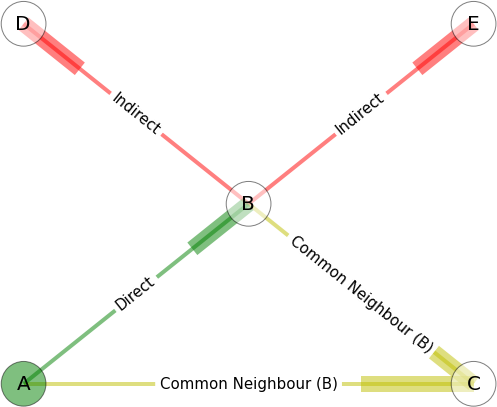
\includegraphics[width=0.6\linewidth]{node_relationships}
              \vspace{1ex}
              \caption{Direct, Recommendation, and Indirect trust relationships}
            \end{figure}

          \end{block}
          %%%%%%%%%%%%
          \begin{block}{The Need for Multi-Domain Trust in Autonomous Systems}
              Communications not the only target for an attacker (or failure);
                \begin{itemize}
                  \item Following to restricted area
                  \item Masquerading
                  \item Hardware Degradation
                  \item Resource attack via propulsive power
                \end{itemize}
            Physical observation presents opportunity to further reduce the available threat surface while also discriminating between 'True' attacks and mechanical failure.
              
            \vspace{0.3\baselineskip}

            Also could provide additional 'handshake' protocols for 'friendly' fleets/teams through reactionary behaviours

            \vspace{0.3\baselineskip}

            Potential attacks exist within a multi-domain threat surface, and as further metrics and domains of trust are included in a TMF, attackers are increasingly restricted in their behaviour until the only way to avoid detection is to behave correctly.
            \begin{figure}[h]
              \centering
              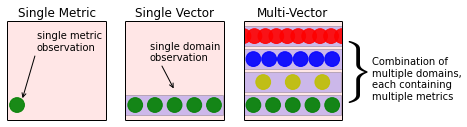
\includegraphics[width=0.9\linewidth]{threat_surface_sum}
              \caption{Threat Surface for Trust Management Frameworks}
            \end{figure}
          \end{block}

   
          %%%%%%%%%%%%
          \iffalse
          \begin{block}{Base Collision avoidance behaviour (Boid-like flocking)}
            \begin{columns}[T]
              \begin{column}{.70 \textwidth}
                Simple Boidean flocking is used to provide a safe 
                \begin{itemize}
                  \item Cohesion
                    \begin{equation}
                      F_{j,C}= F_A\left(p_j, \frac{1}{N}\sum\limits_{\forall i \ne j}^N{p_i}, d_{max}\right)
                    \end{equation}
                  \item Repulsion
                    \begin{equation}
                      F_{j,H}= \sum\limits_{\forall i \ne j}^N F_R\left(p_j, p_i, d_{max}) \big| d_{max}>\|p_i-p_j\|\right)
                    \end{equation}
                  \item Alignment
                    \begin{equation}
                      F_{j,CA}= \frac{1}{N}\cdot\left(\sum\limits_{\forall i \ne j}^N \hat{v_i}\right) 
                    \end{equation}
                \end{itemize}
              \end{column}
              \begin{column}{.25\textwidth}
                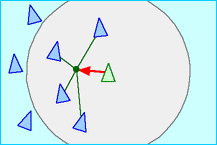
\includegraphics[width=0.9\textwidth]{figures/flocking_cohesion.gif}
                \vspace{0.3\baselineskip}
                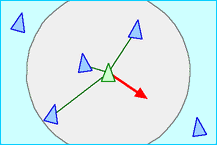
\includegraphics[width=0.9\textwidth]{figures/flocking_separation.gif}
                \vspace{0.3\baselineskip}
                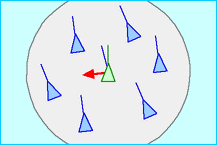
\includegraphics[width=0.9\textwidth]{figures/flocking_alignment.gif}
              \end{column}
            \end{columns}
            \vspace{0.3\baselineskip}
            Where $F_A$ is a scaled vector attraction function, and $F_R$ is an equivalent repulsion function
          \end{block}
          \fi
          %%%%%%%%%%%%
          \begin{block}{Operational Mission Profiles}
            Generic behaviours currently under investigation include:
            \begin{itemize}
              \item \emph{Waypointing} - Attraction to a point or a chain of points, providing pre-described patrol networks
              \item \emph{Surveying} - Fleets can be tasked to provide one-shot, or persistent coverage of an area of the environment utilising a dynamic lawnmower pattern.
              \item \emph{Dynamic Constraint} - Repulsion from a series of points, analogous to sea-borders or shipping lanes.
            \end{itemize}

            Potentially Exploitable Behaviours not yet developed include:
            \begin{itemize}
              \item \emph{Capacity Based Homing} - Where a node leaves and later returns to the fleet, for instance for refuelling or resupply.
              \item \emph{Dynamic Communications Maintenance} - The fleet can adjust to changing communications environments.
            \end{itemize}
          \end{block}
          %%%%%%%%%%%%


          }
        \end{minipage}
      \end{beamercolorbox}
    \end{column}
    % ---------------------------------------------------------%
    % end the column

    % ---------------------------------------------------------%
    % Set up a column 
    \begin{column}{\colwidth}
      \begin{beamercolorbox}[center,wd=\textwidth]{postercolumn}
        \begin{minipage}[T]{.98\textwidth} % tweaks the width, makes a new \textwidth
          \parbox[t]{\textwidth}{ % must be some better way to set the the height, width and textwidth simultaneously
           %%%%%%%%%%%%

            \begin{block}{Malicious Behaviours}
            A series of 'Malicious' behaviours have been designed, where one or more nodes were actively attempting to compromise the fleet in some way.
            \begin{itemize}
              \item \emph{Shadow} - Following the fleet without restricted mission data
              \item \emph{Spy} - A node that intermittently rises in the fleet, potentially surfacing to relay mission information to a third party
              \item \emph{Sloth} - Selfish conservation of energy by taking minimal paths
              \item \emph{Stalker} - Tailing a specific node, attempting to use this consistent history to poision the trust network
              \item \emph{Scoundrel} - Falsely reporting its estimated position with the intention to corrupt a collaborative positioning system or induce a collision
            \end{itemize}

            Additionally, there are non-malicious behaviours, the classification of which is equally important in separating friend from foe.
            \begin{itemize}
              \item \emph{Slow Coach} - Where a node's power train is damaged, causing reduced maneuverability and performance
              \item \emph{Spin Doctor} - Damage to control surfaces or to Inertial Navigation System
            \end{itemize}

          \end{block}

          %%%%%%%%%%%%
          \iffalse
          \begin{block}{Simulation Framework}
            Bespoke Simulation framework consisting of three modules:
            \begin{itemize}
              \item \texttt{Aietes} : the original base behavioural simulator, performing agent-based modelling of the motions of AUV's within an 
                environment
              \item \texttt{Bounos} : a collection of data processing and collation functions.
              \item \texttt{Ephyra} : a GUI visualisation (and later, control) system for both Aietes and Bounos (See Fig~\ref{fig:Ephyra})
            \end{itemize}

            \vspace{0.3\baselineskip}

            It is highly flexible, allowing for:
            \begin{itemize}
              \item Arbitrary node configurations (both in terms of physical and communications capabilities)
              \item Generically Based on the REMUS 100 configuration and physical model, but extendible to other dynamics
              \item Support for runtime and \emph{a-posteriori} statistical analysis with numpy/scipy/pandas
              \item Componentised Behaviour network, with a Boid-like collaborative control path base behaviour (flocking)
              \item Integration to the SUNSET emulation platform, allowing for rapid integration to real equipment
            \end{itemize}
            \vspace{\lineskip}
            \begin{figure}
              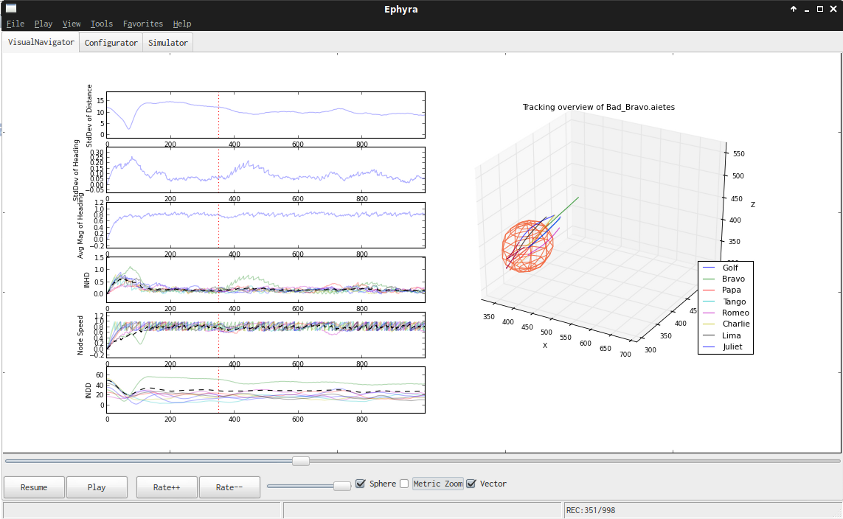
\includegraphics[width=0.9\textwidth]{figures/ephyra_vis}
              \caption{The Ephyra visualiser built with WxPython allows for rapid modelling and analysis of multi-dimensional vector data, in this case showing a interactive real-time 3D model of the fleet positions and trails, as well as overlay information on individual and fleet behaviours, and on the left, fleet- and node- level metrics plotted over time.}
              \label{fig:Ephyra}
            \end{figure}
          \end{block}     
          \fi
          %%%%%%%%%%%%
            
%%%%%%%%%%%%
          \begin{block}{Proof of Concept Analysis}
            
            The aim of the Proof of Concept is to demostrate not only the detection capability of using behavioural metrics to access trust but to differentiate between malicious and impaired bheaviours.

            \vspace{0.3\baselineskip}

            Three fleets are simluated performing a simple patrol mission, each with a particular behaviour set. The first has a malicious node performing a 'Shadow' behaviour, representing a malicious outside actor attempting to infiltrate the fleet. The second has an impaired node exhibiding 'SlowCoach' behaviour, representing a damaged or faulty but otherwise good node. 

            \vspace{0.3\baselineskip}
            
            
            The simulations were run to for a standard eight hour mission time, with three primary metrics being assessed at run time by each node:
            \begin{itemize}
              \item \emph{INHD}: Inter Node Heading Deviation, or the per-node deviation from the fleet-average velocity vector
              \item \emph{Node Speed}: The Magnitude of Velocity of each node
              \item \emph{INDD}: Inter Node Distance Deviation, or the normalised deviation between the inter-node distance matrices from the perspective of each node
            \end{itemize}
            \begin{figure}
              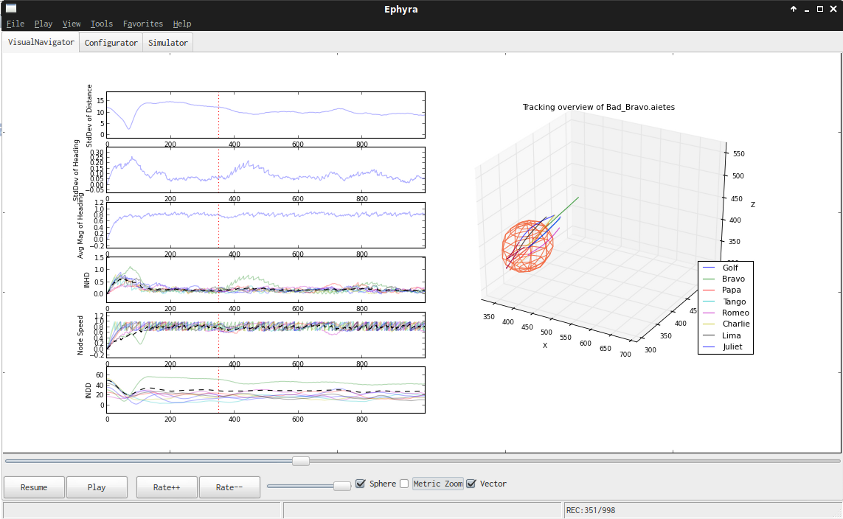
\includegraphics[width=0.8\textwidth]{figures/ephyra_vis}
              \caption{The Ephyra visualiser allows for rapid modelling and analysis of node data, as well as overlay information on individual and fleet behaviours and metrics.}
              \label{fig:Ephyra}
            \end{figure}
            In this model, there are no 'positive' trust demonstrations, so all nodes are 'distrusted' to some degree or 'untrusted'. This distrust is dependant on consistent or periodic deviation from fleet norms. This trust assessment is developed by each individual node against each other node, however for this Proof of Concept, a global metric state was used (free of environmental and positional drift factors).

            \end{block}

%%%%%%%%%%%%
          }
          % ---------------------------------------------------------%
          % end the column
          \end{minipage}
        \end{beamercolorbox}
      \end{column}
      % ---------------------------------------------------------%

    % ---------------------------------------------------------%
    % Set up a column 
    \begin{column}{\colwidth}
      \begin{beamercolorbox}[center,wd=\textwidth]{postercolumn}
        \begin{minipage}[T]{.98\textwidth} % tweaks the width, makes a new \textwidth
          \parbox[t]{\textwidth}{ % must be some better way to set the the height, width and textwidth simultaneously
            % Since all columns are the same length, it is all nice and tidy.  You have to get the height empirically
            % ---------------------------------------------------------%
            % fill each column with content

            \begin{block}{Analysis Cont.}
                      \begin{figure}
              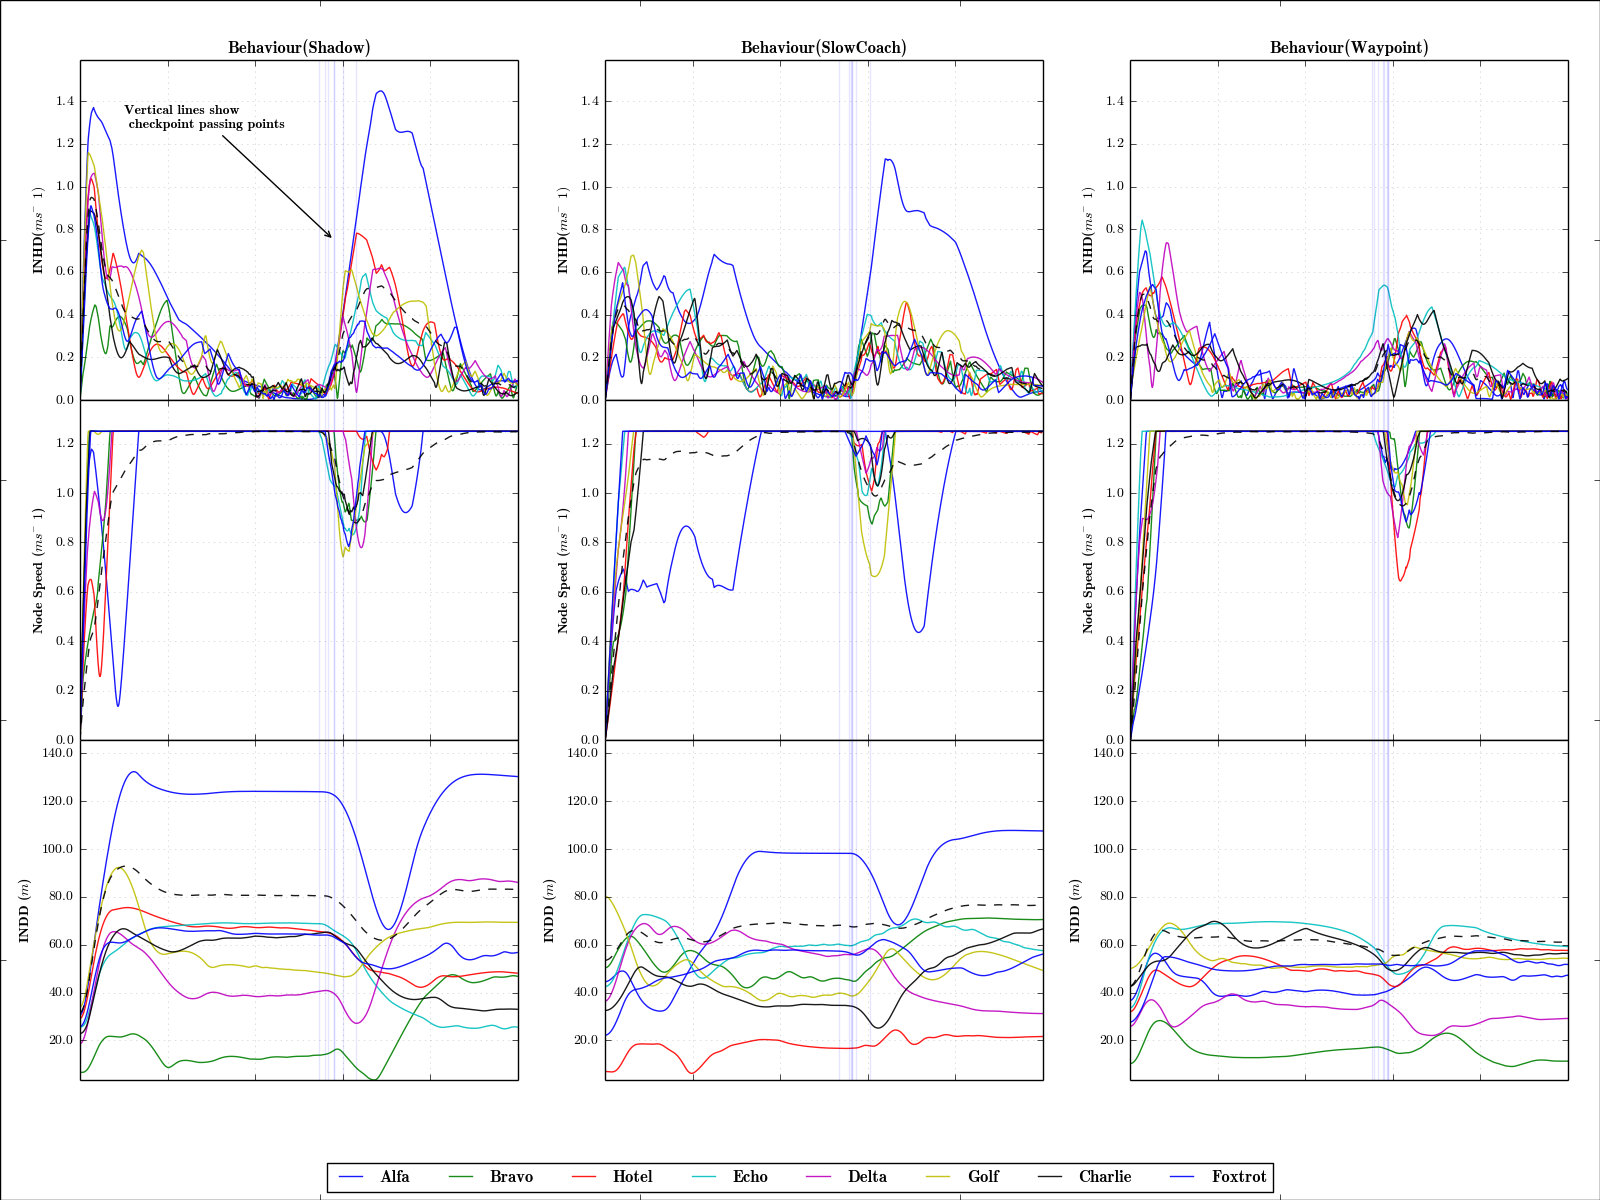
\includegraphics[width=0.9\textwidth]{figures/BehaviourMetricComparison}
              \caption{Per-Simulation metric measurements for Malicious, Impaired, and Control behaviours (Shadow, SlowCoach and Waypoint)}
              \label{fig:Bad_Alfa_Comparison}
            \end{figure}

            \emph{INDD} is an obvious candidate for a suspicion 'trigger', but looking at \emph{INHD} values after a few hundred seconds of simulation time; an anomaly is clearly being detected. 

            \vspace{0.3\baselineskip}

            In addition, \emph{Alfa} node (the Blue Line) is clearly an outlier in terms of \emph{INHD} and \emph{Node Speed} in the earliest sections of the graph, at which point nothing appears to be out of the ordinary in \emph{INDD}. This implies that a fusion of metrics would be more effective than a simple detection envelope on a single metric.

            \begin{figure}
              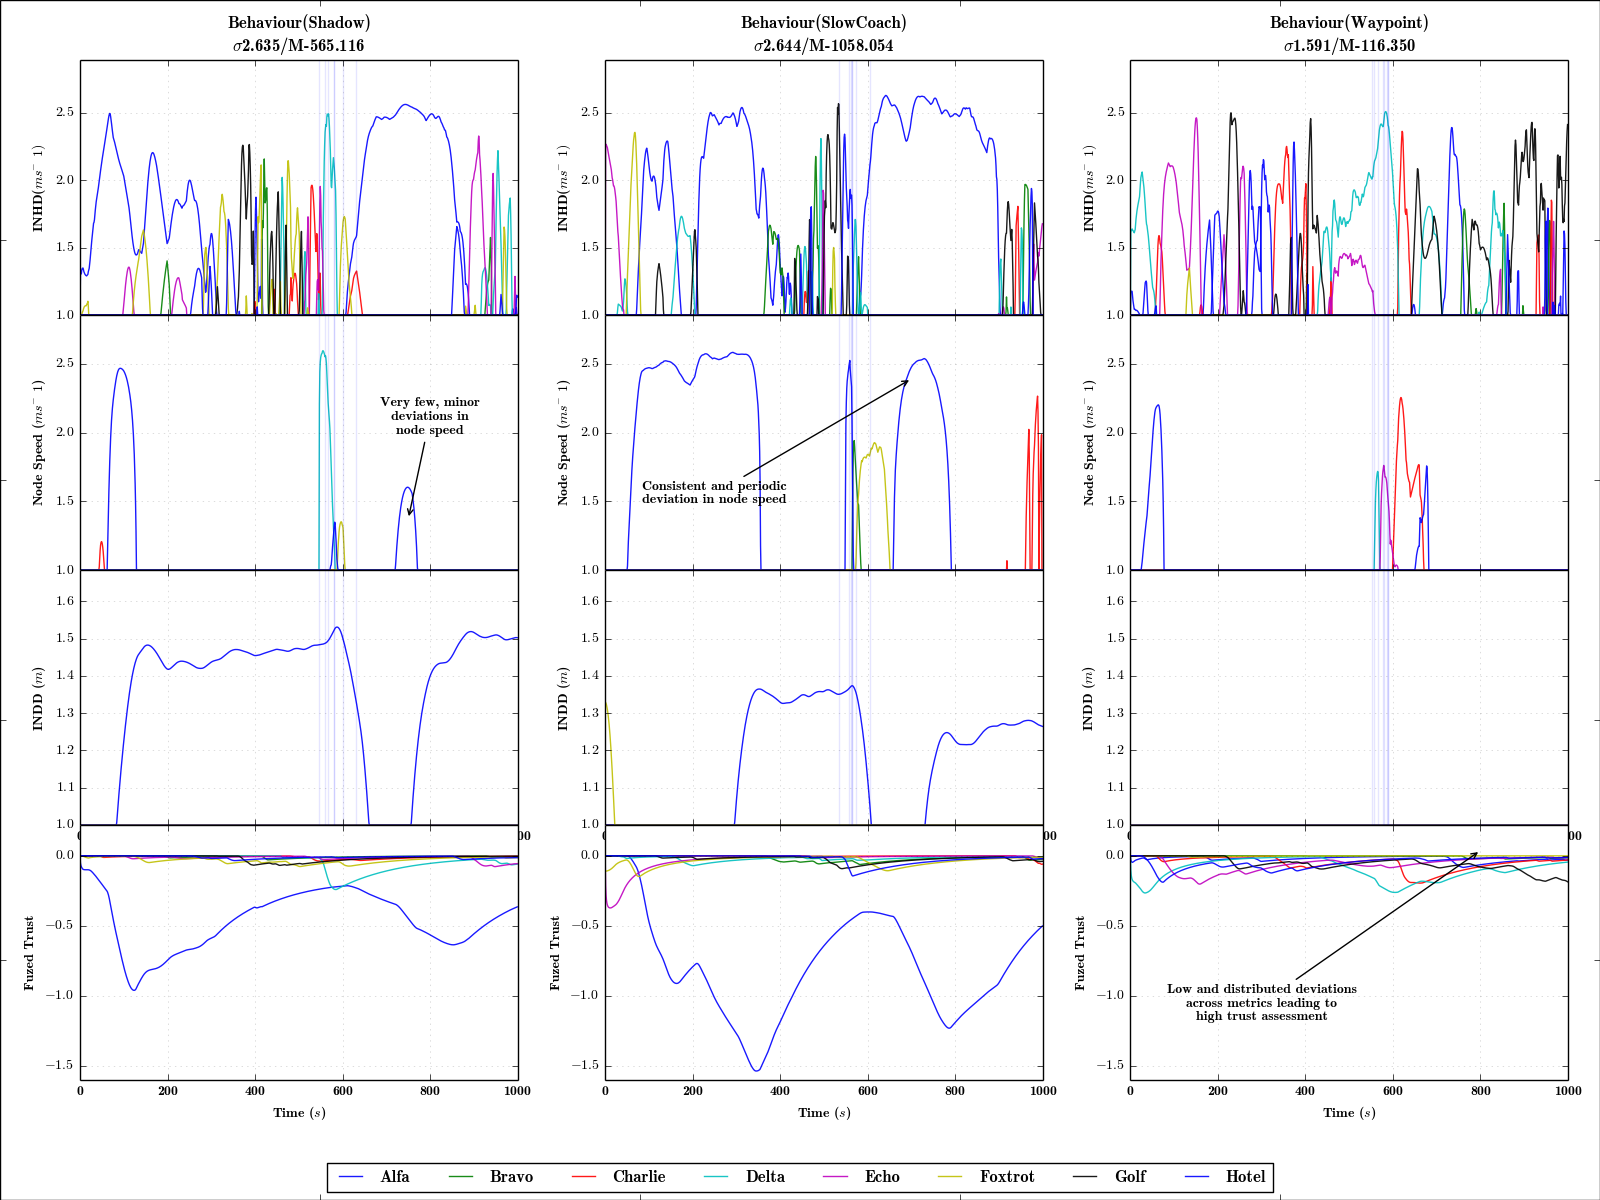
\includegraphics[width=0.9\textwidth]{figures/Bad_Alfa_Fusion}
              \caption{Per-Node deviations for each metric, with an additional row showing an EWMA based cross-metric trust assessment. Note the different in 'Node Speed' triggers between the malicious and impaired behaviours }
              \label{fig:Bad_Alfa_Fusion}
            \end{figure}


            Considering the Baseline data (Right side of Figure ~\ref{fig:Bad_Alfa_Comparison}), it's clear that these metrics are not infallible, as is demonstrated by the number of relatively short-lived false positives, demonstrating the need to use multiple metrics for reliable trust assessment.

            \vspace{0.3\baselineskip}

            Figure ~\ref{fig:Bad_Alfa_Fusion} demonstrates a windowed, weighted trust fusion, where deviations in individual metrics are combined to generate a Trust Value. 
          \end{block}

          %%%%%%%%%%%%
            \begin{block}{Future Applications}
              \begin{itemize}
                \item Due to the high communications, motion, and computation costs, and lack of external location reporting (\emph{e.g. GPS}), 
                  behavioural analysis in the marine environment is particularly difficult, but if successful, can be reliably applied in a wide 
                  variety of fields including but not limited to
                \begin{itemize}
                  \item Self-Driving Cars
                  \item Environmental Survey drones (terrestrial, marine, and aerial)
                  \item Satellite Communications Arrays
                  \item Internet Certificate Authority verification
                  \item Verifiable Distributed Computing
                \end{itemize}
              \end{itemize}              
            \end{block}
%%%%%%%%%%%%

          }
          % ---------------------------------------------------------%
          % end the column
        \end{minipage}
      \end{beamercolorbox}
    \end{column}
    % ---------------------------------------------------------%
    % end the column   % end the column
    % ---------------------------------------------------------%
    % Set up a column 
    \begin{column}{\colwidth}
      \begin{beamercolorbox}[center,wd=\textwidth]{postercolumn}
        \begin{minipage}[T]{.98\textwidth} % tweaks the width, makes a new \textwidth
          \parbox[t]{\textwidth}{ % must be some better way to set the the height, width and textwidth simultaneously
          % Since all columns are the same length, it is all nice and tidy.  You have to get the height empirically
          % ---------------------------------------------------------%
          % fill each column with content
          %%%%%%%%%%%%

            \begin{block}{Conclusions}
              This research area presents a range of challenges and opportunities within both civil and defence operations; an auditable trust framework for automated marine craft would be a significant enabling factor to the roll-out of more low-maintenance or even ``Fire and Forget'' deployments for persistent patrol/monitoring tasks. 

              \vspace{0.3\baselineskip}

              Open Hypotheses in this field that this project intends to answer are:
              \begin{itemize}
                \item How can optimality in trust assessment based on behaviour be defined win a distributed, dynamic network topology?
                \item Is there a quantifiable benefit to cross-domain comparison beyond single-vector trust? (i.e. 1-D vector vs cross domain comparison)
                \item Is there an optimal \emph{generic} cross domain fusion methodology?
              \end{itemize}
            \end{block}
%%%%%%%%%%%%
          \begin{block}{Current Publications}
            \begin{itemize}
              \item A Multi-Vector Trust Framework for Autonomous Systems \cite{Bolster2014}
                \begin{itemize}
                  \item Symposium paper to the Association for the Advancement of Artificial Intelligence on the current state of work, presenting our progress towards multi-vector trust
                \end{itemize}


              \item Analysis of Trust Interfaces in Autonomous and Semi-Autonomous Collaborative MHPC Operations \cite{Bolster2014a}
                \begin{itemize}
                  \item Part of a Five-Eyes defence strategy programme (TTCP) for assuring C3I capabilities as part of FF2020
                \end{itemize}

            \end{itemize}


          \end{block}

          %%%%%%%%%%%%
          \begin{block}{Development Plan}
            \begin{itemize}
              \item Behaviour Detection (Q3 14) - Formal Analysis of Behavioural Trust Systems
                \begin{itemize}
                  \item ASON 2014 : Seventh Int. WS on Autonomous Self-Organizing Networks (Aug 14)
                  \item AHUC 2014 : The Fourth Int. WS on Ad Hoc and Ubiquitous Computing (Aug 14)
                  \item ICCAR 2015 : WASET Int. Conf. on Control, Automation and Robotics (Dec 14)
                \end{itemize}
              \item MANET/Marine comparison (Q4 14) - Formal Comparison between Terrestrial MANET / Marine contexts
              \item Multi-Domain Trust Assessment (Q4 14) - Combination of Communicative and Physical Behaviour Trusts
                \begin{itemize}
                  \item IEEE Trans. on Communications / Dependable and Secure Computing / Intelligent Systems
                \end{itemize}
              \item Reactionary/Perturbative Trust (Q1 15) - Exploration of reactionary behaviours for teams to 'shake down' suspects
                \begin{itemize}
                  \item SASO15:Self-Adaptive and Self-Organizing Systems, 
                  \item SEAMS15: Software Engineering for Adaptive and Self-Managing Systems
                \end{itemize}
            \end{itemize}

          \end{block}


          %%%%%%%%%%%%


            \begin{block}{Bibliography}

              \printbibliography[title=References]% [nottype=video]}
            \end{block}
            }
          % ---------------------------------------------------------%
          % end the column
        \end{minipage}
      \end{beamercolorbox}
    \end{column}
    % ---------------------------------------------------------%
    % end the column   % end the column

  \end{columns}
\end{frame}
\end{document}


%%%%%%%%%%%%%%%%%%%%%%%%%%%%%%%%%%%%%%%%%%%%%%%%%%%%%%%%%%%%%%%%%%%%%%%%%%%%%%%%%%%%%%%%%%%%%%%%%%%%
%%% Local Variables: 
%%% mode: latex
%%% TeX-PDF-mode: t
%%% End:
